%%%%%%%%%%%%%%%%%%%%%%%%%%%%%%%%%%%%%%%%%%%
%
% From a template maintained at https://github.com/jamesrobertlloyd/cbl-tikz-poster
%
% Code near the top should be fairly standard and not need to be changed
%  - except for the document class
% Code lower down is more likely to be customised
%
%%%%%%%%%%%%%%%%%%%%%%%%%%%%%%%%%%%%%%%%%%%

%%%%%%%%%%%%%%%%%%%%%%%%%%%%%%%%%%%%%%%%%%%
%
% Document class
%
% Change this if you want a different size / orientation poster etc
%
%%%%%%%%%%%%%%%%%%%%%%%%%%%%%%%%%%%%%%%%%%%

%\documentclass[landscape,a0b,final,a4resizeable]{a0poster}
\documentclass[portrait,a0b,final,a4resizeable]{a0poster}
%\documentclass{article}
%\usepackage[portrait,a0paper,margin=1in]{geometry}

\addtolength{\oddsidemargin}{-1.2in}
%	\addtolength{\evensidemargin}{-.875in}

%%%%%%%%%%%%%%%%%%%%%%%%%%%%%%%%%%%%%%%%%%%
%
% 'Basic' packages
%
% TODO - Almost certainly some are unnecessary - feel free to remove nonstandard
% packages if you think it is a good idea not to always have them
%
%%%%%%%%%%%%%%%%%%%%%%%%%%%%%%%%%%%%%%%%%%%


\usepackage{multicol}
\usepackage{color}
%\usepackage{shadow}
\usepackage{morefloats}
%\usepackage{cite}
\usepackage[pdftex]{graphicx}
\usepackage{rotating}
\usepackage{amsmath, amsthm, amssymb, bm}
\usepackage{array}
%\usepackage{nth}
%\usepackage[square,numbers]{natbib}
\usepackage{booktabs}
\usepackage{multirow}
\usepackage{hyperref}

%%%%%%%%%%%%%%%%%%%%%%%%%%%%%%%%%%%%%%%%%%%
%
% TIKZ packages and common definitions
%
% Add extra things as per your tikz needs
%
%%%%%%%%%%%%%%%%%%%%%%%%%%%%%%%%%%%%%%%%%%%

\usepackage{../common/picins}
\usepackage{tikz}
\usetikzlibrary{shapes.geometric,arrows,chains,matrix,positioning,scopes,calc}
\tikzstyle{mybox} = [draw=white, rectangle]

%%%%%%%%%%%%%%%%%%%%%%%%%%%%%%%%%%%%%%%%%%%
%
% myfig
%
% \myfig - replacement for \figure
% necessary, since in multicol-environment 
% \figure won't work        
%                 
%%%%%%%%%%%%%%%%%%%%%%%%%%%%%%%%%%%%%%%%%%%

\newcommand{\myfig}[3][0]{
\begin{center}
  \vspace{1.5cm}
  \includegraphics[width=#3\hsize,angle=#1]{#2}
  \nobreak\medskip
\end{center}}

%%%%%%%%%%%%%%%%%%%%%%%%%%%%%%%%%%%%%%%%%%%
%
% mycaption                
%
% \mycaption - replacement for \caption
% necessary, since in multicol-environment \figure and
% therefore \caption won't work
%
%%%%%%%%%%%%%%%%%%%%%%%%%%%%%%%%%%%%%%%%%%%

%\newcounter{figure}
\setcounter{figure}{1}
\newcommand{\mycaption}[1]{
  \vspace{0.5cm}
  \begin{quote}
    {{\sc Figure} \arabic{figure}: #1}
  \end{quote}
  \vspace{1cm}
  \stepcounter{figure}
}

%%%%%%%%%%%%%%%%%%%%%%%%%%%%%%%%%%%%%%%%%%%
%
% Some standard colours
%
%%%%%%%%%%%%%%%%%%%%%%%%%%%%%%%%%%%%%%%%%%%

\definecolor{camlightblue}{rgb}{0.601 , 0.8, 1}
\definecolor{camdarkblue}{rgb}{0, 0.203, 0.402}
\definecolor{camred}{rgb}{1, 0.203, 0}
\definecolor{camyellow}{rgb}{1, 0.8, 0}
\definecolor{lightblue}{rgb}{0, 0, 0.80}
\definecolor{white}{rgb}{1, 1, 1}
\definecolor{whiteblue}{rgb}{0.80, 0.80, 1}

%%%%%%%%%%%%%%%%%%%%%%%%%%%%%%%%%%%%%%%%%%%
%
% Some look and feel definitions
%
%%%%%%%%%%%%%%%%%%%%%%%%%%%%%%%%%%%%%%%%%%%

\setlength{\columnsep}{0.03\textwidth}
\setlength{\columnseprule}{0.0018\textwidth}
\setlength{\parindent}{0.0cm}

%%%%%%%%%%%%%%%%%%%%%%%%%%%%%%%%%%%%%%%%%%%
%
% \mysection - replacement for \section*
% 
% Puts a pretty box around some text
% TODO - any other thoughts for what this box should look like
%
%%%%%%%%%%%%%%%%%%%%%%%%%%%%%%%%%%%%%%%%%%%

\tikzstyle{mysection} = [rectangle, 
									draw=none, 
									shade, 
									outer color=camlightblue!30,
									inner color=camlightblue!30,
									text width=0.965\columnwidth,
									text centered,
									rounded corners=20pt,
									minimum height=0.11\columnwidth]

\newcommand{\mysection}[1]
{
\begin{center}
  \begin{tikzpicture}
    \node[mysection] {\sffamily\bfseries\LARGE#1};
  \end{tikzpicture}
\end{center}
}

%%%%%%%%%%%%%%%%%%%%%%%%%%%%%%%%%%%%%%%%%%%
%
% Set the font
%
% TODO - Not sure what a canonical choice is - feel free to modify
%
%%%%%%%%%%%%%%%%%%%%%%%%%%%%%%%%%%%%%%%%%%%

\renewcommand{\familydefault}{cmss}
\sffamily

%%%%%%%%%%%%%%%%%%%%%%%%%%%%%%%%%%%%%%%%%%%
%
% Poster environment
%
% Centres everything and can be used to define the width of the content
%
%%%%%%%%%%%%%%%%%%%%%%%%%%%%%%%%%%%%%%%%%%%

\newenvironment{poster}{
  \begin{center}
  \begin{minipage}[c]{0.95\textwidth}
}{
  \end{minipage} 
  \end{center}
}

%%%%%%%%%%%%%%%%%%%%%%%%%%%%%%%%%%%%%%%%%%%
%
% This is probably a good place to put content specific packages and definitions
%
%%%%%%%%%%%%%%%%%%%%%%%%%%%%%%%%%%%%%%%%%%%

\usepackage{preamble}
\usepackage{tabularx}

\def\newarrow{\mbox{\begin{tikzpicture}
             \useasboundingbox{(-3pt,-4.5pt) rectangle (19pt,1pt)};
             \draw[->] (0,-0.07)--(17pt,-0.07);\end{tikzpicture}}}

%%%%%%%%%%%%%%%%%%%%%%%%%%%%%%%%%%%%%%%%%%%
%
% The document environment starts here
%
%%%%%%%%%%%%%%%%%%%%%%%%%%%%%%%%%%%%%%%%%%%

\begin{document}

%%%%%%%%%%%%%%%%%%%%%%%%%%%%%%%%%%%%%%%%%%%
%
% Begin the poster environment - centres things and potentially changes the width
%
%%%%%%%%%%%%%%%%%%%%%%%%%%%%%%%%%%%%%%%%%%%

\begin{poster}

%%%%%%%%%%%%%%%%%%%%%%%%%%%%%%%%%%%%%%%%%%%
%
% Potentially add some space at the top of the poster
%
%%%%%%%%%%%%%%%%%%%%%%%%%%%%%%%%%%%%%%%%%%%

\vspace{0\baselineskip}

%%%%%%%%%%%%%%%%%%%%%%%%%%%%%%%%%%%%%%%%%%%
%
% Draw the header as a TIKZ picture
%
% Using TIKZ to allow for easy alignment
%
%%%%%%%%%%%%%%%%%%%%%%%%%%%%%%%%%%%%%%%%%%%

\begin{center}
\hspace{-1cm}
\begin{tikzpicture}[x=0.5\textwidth]
    % Dummy nodes at edges for spacing
    % TODO - a better way?
    %\node at (+1, 0) {};    
    %\node at (-1, 0) {};
    % Set the size of the badges
    \def \badgeheight {0.1\textwidth}
    % Title text
    \node[inner sep=0,text width=0.7\textwidth,text centered,font=\Huge] (Title) at (0,0) 
    {
      {\sffamily \Huge \textbf{Structure Discovery in Nonparametric Regression through \\ Compositional Kernel Search}}\\
      {\huge\sffamily David Duvenaud, James Robert Lloyd, Roger Grosse,
      }\\      \vspace{-0.1\baselineskip} {\huge\sffamily 
      Joshua B. Tenenbaum, Zoubin Ghahramani}\\
     % \vspace{-0.3\baselineskip}
     % {\large\sffamily 1: Department of Engineering, University of Cambridge, UK 2: Massachusetts Institute of Technology, USA}
    };
    % Cambridge badge
    \node [mybox] (Cambridge Badge) at (+0.85, 0) {
        \includegraphics[height=\badgeheight]{../badges/cam-crest-and-text.pdf}
    };
    % CBL badge
    %\node [mybox] (CBL Badge) at (+0.9, 0) {
    %    
\includegraphics[height=\badgeheight]{../badges/cbl-badge-cropped.png}
    %};
    % MIT badge
    \node [mybox] (MIT Badge) at (-0.85, 0) {
        
\includegraphics[height=\badgeheight]{../badges/MIT2.jpg}
    };
    % QR code
    %\node [mybox] (QR code) at (-0.95, 0) {
    %    
\includegraphics[height=\badgeheight]{../badges/QR.png}
    %};
\end{tikzpicture}
\end{center}

%%%%%%%%%%%%%%%%%%%%%%%%%%%%%%%%%%%%%%%%%%%
%
% Spacing between title and main body
%
%%%%%%%%%%%%%%%%%%%%%%%%%%%%%%%%%%%%%%%%%%%

\vspace{1\baselineskip}

%%%%%%%%%%%%%%%%%%%%%%%%%%%%%%%%%%%%%%%%%%%
%
% Columns environment
%
%%%%%%%%%%%%%%%%%%%%%%%%%%%%%%%%%%%%%%%%%%%

\begin{multicols}{2}

%%%%%%%%%%%%%%%%%%%%%%%%%%%%%%%%%%%%%%%%%%%
%
% Start of content
%
%%%%%%%%%%%%%%%%%%%%%%%%%%%%%%%%%%%%%%%%%%%

\large


%\mysection{Data often exhibits high level structure or patterns}

%\vspace{0\baselineskip}

%\begin{center}
%  \begin{tikzpicture}%[transform canvas={scale = 0.9}]
  \begin{scope}[yshift=0\textwidth]
    \begin{scope}[xshift=-0.08\textwidth]
      \node [mybox] (all) at (0, 0) {
        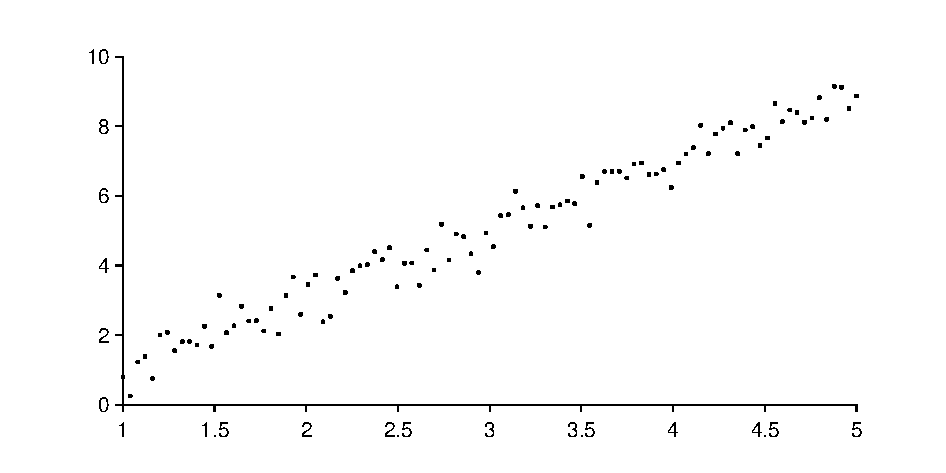
\includegraphics[width=0.13\textwidth]{../figures/linear.pdf}
      };
    \end{scope}
    \begin{scope}[xshift=+0.08\textwidth]
      \node [mybox] (all) at (0, 0) {
        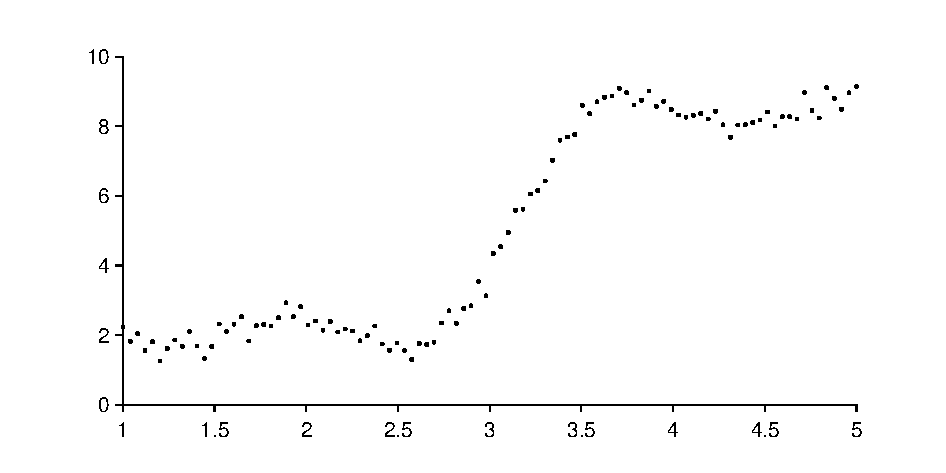
\includegraphics[width=0.13\textwidth]{../figures/periodic.pdf}
      };
    \end{scope}
  \end{scope}
  \begin{scope}[yshift=-0.065\textwidth]
    \begin{scope}[xshift=-0.08\textwidth]
      \node [mybox] (all) at (0, 0) {
        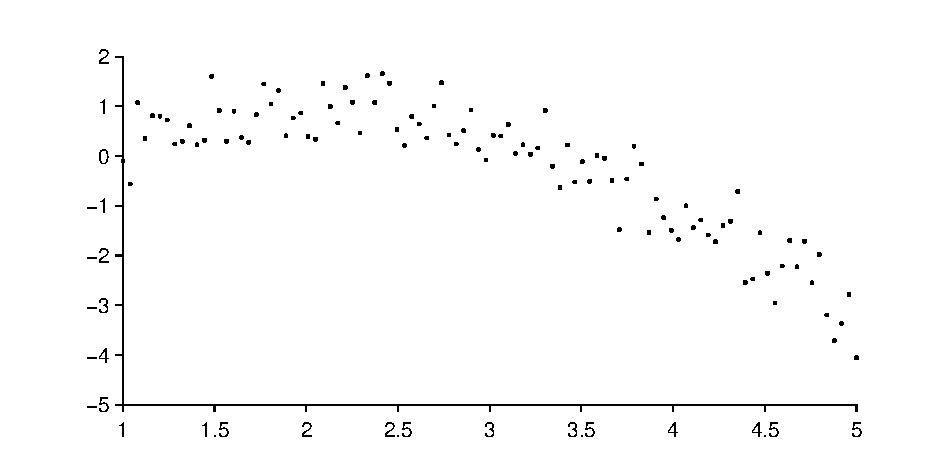
\includegraphics[width=0.13\textwidth]{../figures/quadratic.pdf}
      };
    \end{scope}
    \begin{scope}[xshift=+0.08\textwidth]
      \node [mybox] (all) at (0, 0) {
        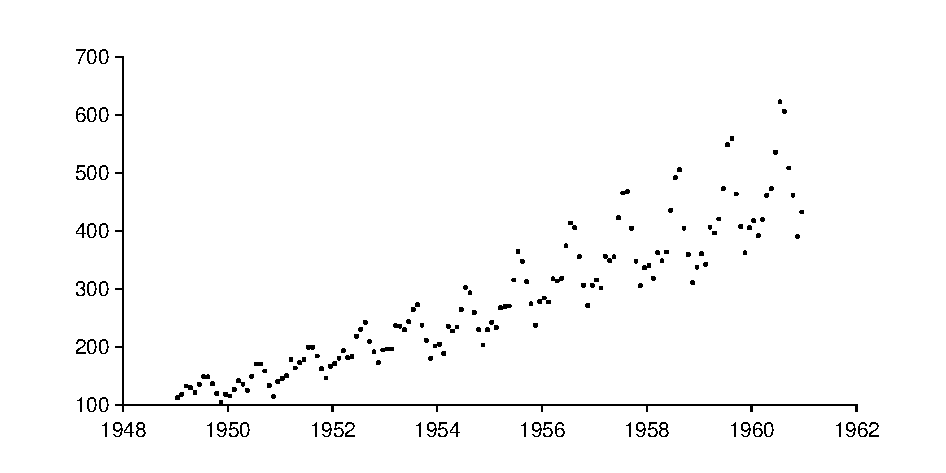
\includegraphics[width=0.13\textwidth]{../figures/airline.pdf}
      };
    \end{scope}
  \end{scope}
\end{tikzpicture}


%\end{center}

%\vspace{0\baselineskip}

%\begin{itemize}
%  \item Traditionally, a researcher / scientist / statistician would select an appropriate model for the type of structures present
%  \item Automatic model selection techniques already exist, typically choosing between a finite or restricted set of models
%  \item Instead, we automate statistical model \emph{construction}%, which allows for a very large set of models to be considered
%\end{itemize}

%\vspace{0.5\baselineskip}

\mysection{Identifying structure is crucial for extrapolation}

\vspace{0\baselineskip}

\begin{center}
  \begin{tikzpicture}%[transform canvas={scale = 0.9}]
  \begin{scope}[yshift=0\textwidth]
    \begin{scope}[xshift=-0.08\textwidth]
      \node [mybox] at (0, 0) {
        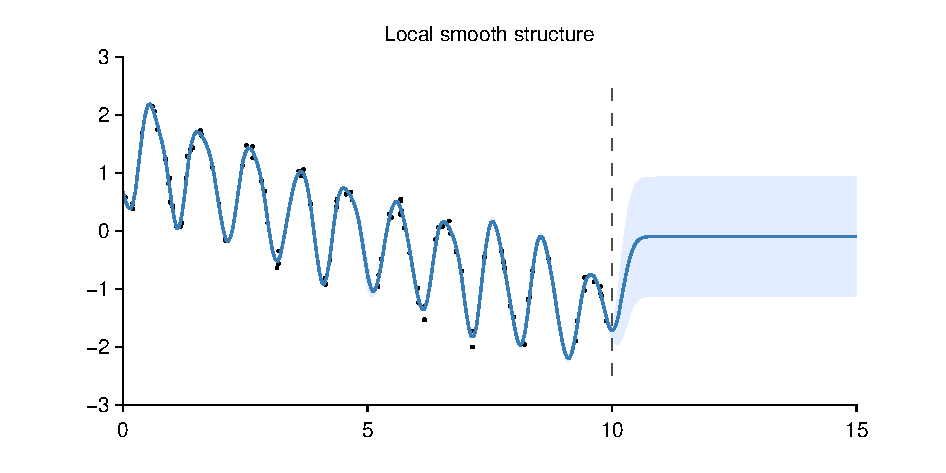
\includegraphics[width=0.13\textwidth]{../figures/synth_extrap_bad.pdf}
      };
    \end{scope}
    \begin{scope}[xshift=+0.08\textwidth]
      \node [mybox] at (0, 0) {
        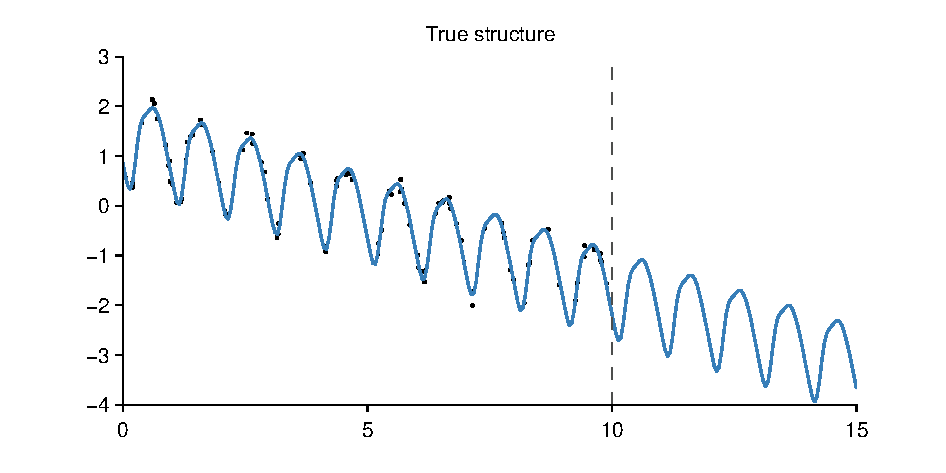
\includegraphics[width=0.13\textwidth]{../figures/synth_extrap_good.pdf}
      };
    \end{scope}
  \end{scope}
\end{tikzpicture}


\end{center}

\vspace{0\baselineskip}



\begin{itemize}
  \item Traditionally, a statistician proposes an appropriate model for the type of structures present
  \item Automatic model selection techniques already exist, typically choosing between a finite or restricted set of models
  \item Instead, we automate statistical model \emph{construction}%, which allows for a very large set of models to be considered
\end{itemize}

\vspace{0.5\baselineskip}

\mysection{Gaussian processes model structure through kernels}

\vspace{0.5\baselineskip}

\begin{itemize}
  \item The kernel specifies which structures are likely under the \gp{} prior, which in turn determines the generalization properties of the model.
  \item Below we list standard base kernels, and draws from the corresponding \gp{} priors:
\end{itemize}
\vspace{1\baselineskip}
\newcommand{\fhbig}{5.0cm}
\newcommand{\fwbig}{5.625cm}
\newcommand{\kernpic}[1]{\includegraphics[height=\fhbig,width=\fwbig]{../figures/structure_examples/#1}}
\newcommand{\kernpicr}[1]{\rotatebox{90}{\includegraphics[height=\fwbig,width=\fhbig]{../figures/structure_examples/#1}}}
\newcommand{\addkernpic}[1]{{\includegraphics[height=\fhbig,width=\fwbig]{../figures/additive_multi_d/#1}}}
\newcommand{\largeplus}{\tabbox{{\Large+}}}
\newcommand{\largeeq}{\tabbox{{\Large=}}}
\newcommand{\largetimes}{\tabbox{{\Large$\times$}}}
\centering
\renewcommand{\tabularxcolumn}[1]{>{\arraybackslash}m{#1}}
%\begin{tabular}{m{\fwbig}m{0.01\textwidth}m{\fwbig}m{0.01\textwidth}m{\fwbig}m{\fwbig}m{\fwbig}}
%\begin{tabular}{C{\fwbig}C{\fwbig}C{\fwbig}C{\fwbig}}%{m{\fwbig}m{\fwbig}m{\fwbig}}
\begin{tabularx}{0.8\columnwidth}{XXXX}
%Composite & Draws from \gp{} & \gp{} posterior \\ \toprule
  \kernpic{se_kernel_draws} & \kernpic{per_kernel_draws_s2} & \kernpic{lin_kernel_draws} & \kernpic{rq_kernel_draws} \\
  {\small \kSE} & {\small \kPer} & {\small \kLin} & {\small \kRQ} \\
  {\small local variation} & {\small repeating structure} & {\small linear functions} & {\small multi-scale variation} \\

%  {\small Squared-exp (\kSE)} & {\small local variation} 
%& {\small Periodic (\kPer)} & {\small repeating structure}
%\\
%\midrule
  
%& \kernpic{rq_kernel} & 
%\\
%  {\small Linear (\kLin)} & {\small linear functions} 
%& {\small Rational-quadratic (\kRQ)} & {\small multi-scale variation}
\end{tabularx}


\vspace{0.5\baselineskip}

\mysection{Kernels can be Composed
% to create more complicated structural assumptions
}

\vspace{0.5\baselineskip}

\begin{itemize}
    \item Constructing appropriate composite kernels has previously been done by  experts
\end{itemize}
\vspace{1\baselineskip}
\centering
\renewcommand{\tabularxcolumn}[1]{>{\arraybackslash}m{#1}}
%\begin{tabular}{m{\fwbig}m{0.01\textwidth}m{\fwbig}m{0.01\textwidth}m{\fwbig}m{\fwbig}m{\fwbig}}
%\begin{tabular}{C{\fwbig}C{\fwbig}C{\fwbig}C{\fwbig}}%{m{\fwbig}m{\fwbig}m{\fwbig}}
\begin{tabularx}{0.8\columnwidth}{XXXX}
  { $\kLin \times \kLin$} & { $\kSE \times \kPer$} & { $\kLin + \kPer$} & { $\kSE + \kPer$ } \\
  \kernpic{lin_times_lin_draws} & \kernpic{se_times_per_draws_s7} & \kernpic{lin_plus_per_draws} & \kernpic{se_plus_per_draws_s7} \\
  { quadratic \newline functions} & { locally \newline periodic} & { periodic \newline with trend} & { periodic \newline with noise} \\
\end{tabularx}




\vspace{1\baselineskip}
\mysection{\ldots defining a rich, open-ended set of models}

\vspace{0.25\baselineskip}

\begin{itemize}
  \item We consider all algebraic expressions composed a small number of base kernels and the operations `$+$' and `$\times$'
  %\item These operations are interpretable\ldots
  %\begin{itemize}
  %  \item Addition of kernels corresponds to the addition of independent functions
  %  \item Multiplication of kernels behaves like an `AND' operation, combining properties of the base kernels
  %\end{itemize}
  %\item \ldots and produce a rich space including many standard statistical models
\end{itemize}

\vspace{0.5\baselineskip}
\paragraph{\large Special cases of our model}
\begin{center}
  \begin{tabular}{l|l}
  Bayesian linear regression & $\Lin$ \\
  %Bayesian quadratric regression & $\Lin \times \Lin$ \\
  Bayesian polynomial regression & $\Lin \times \Lin \times \ldots$\\
  Generalized Fourier decomposition & $\Per + \Per + \ldots$ \\
  Generalized additive models & $\sum_{d=1}^D \SE_d$ \\
  Automatic relevance determination & $\prod_{d=1}^D \SE_d$ \\
  Linear trend with local deviations & $\Lin + \SE$ \\
  Linearly growing amplitude & $\Lin \times \SE$
  \end{tabular}
\end{center}

%\vspace{1\baselineskip}
\newpage

\mysection{\ldots by a greedy search%, \\ producing progressively better models
}

\vspace{0.25\baselineskip}

\begin{itemize}
  \item We try all base kernels, selecting the one with the highest (approximate) marginal likelihood which balances data fit and model complexity
  \item The search continues by adding an extra term to the current best kernel, stopping when marginal likelihood no longer improves
\end{itemize}

\begin{center}
  \begin{tikzpicture}
[sibling distance=0.23\columnwidth,-,thick, level distance=0.1\columnwidth, transform canvas={scale = 0.9}]
%\footnotesize
\node[shape=rectangle,draw,thick,fill=camlightblue!30] {No structure}
  child {node {$\SE$}
  }
  child {node[shape=rectangle,draw,thick,fill=camlightblue!30] {$\RQ$}
    [sibling distance=0.16\columnwidth]
    child {node {$\SE$ + \RQ}}
    child {node {\ldots}}
    child {node[shape=rectangle,draw,thick,fill=camlightblue!30] {$\Per + \RQ$}
      [sibling distance=0.2\columnwidth]
      child {node {$\SE + \Per + \RQ$}}
      child {node {\ldots}}
      child {node[shape=rectangle,draw,thick,fill=camlightblue!30] {$\SE \times (\Per + \RQ)$}
        [sibling distance=0.14\columnwidth]
        child {node {\ldots}}
        child {node {\ldots}}
        child {node {\ldots}}
      }
      child {node {\ldots}}
    }
    %child {node {$\RQ \times \SE$}}
    child {node {\ldots}}
    child {node {$\Per \times \RQ$}}
  }
  child {node {$\Lin$}
  }
  child {node {$\Per$}
  };
\end{tikzpicture}


\end{center}

\vspace{12\baselineskip}

\begin{center}
  %\begin{tikzpicture}[transform canvas={scale = 0.9}]
  \begin{scope}[yshift=0\textwidth]
    \begin{scope}[xshift=-0.08\textwidth]
      \node [mybox] (all) at (0, 0) {
        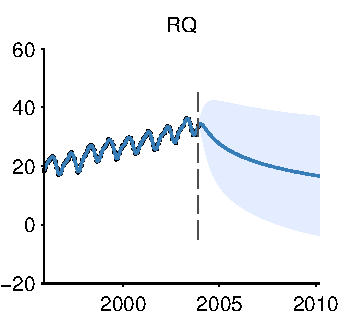
\includegraphics[width=0.13\textwidth]{../figures/11-Feb-v4-03-mauna2003-s_max_level_0/03-mauna2003-s_all_small.pdf}
      };
    \end{scope}
    \begin{scope}[xshift=+0.08\textwidth]
      \node [mybox] (all) at (0, 0) {
        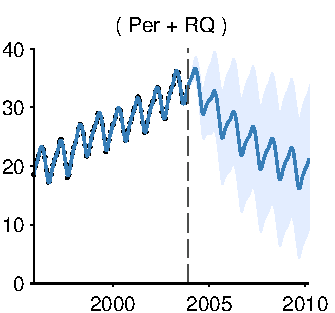
\includegraphics[width=0.13\textwidth]{../figures/11-Feb-v4-03-mauna2003-s_max_level_1/03-mauna2003-s_all_small.pdf}
      };
    \end{scope}
  \end{scope}
  \begin{scope}[yshift=-0.2\textwidth]
  \end{scope}
  \begin{scope}[yshift=-0.13\textwidth]
    \begin{scope}[xshift=-0.08\textwidth]
      \node [mybox] (all) at (0, 0) {
        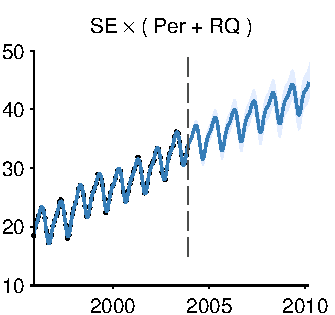
\includegraphics[width=0.13\textwidth]{../figures/11-Feb-v4-03-mauna2003-s_max_level_2/03-mauna2003-s_all_small.pdf}
      };
    \end{scope}
    \begin{scope}[xshift=+0.08\textwidth]
      \node [mybox] (all) at (0, 0) {
        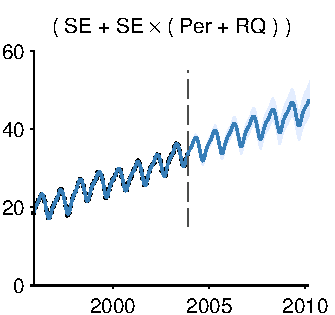
\includegraphics[width=0.13\textwidth]{../figures/11-Feb-v4-03-mauna2003-s_max_level_3/03-mauna2003-s_all_small.pdf}
      };
    \end{scope}
  \end{scope}
\end{tikzpicture}


  \begin{tabular}{cccc}
  Depth 1 & Depth 2 & Depth 3 & Depth 4 \\
          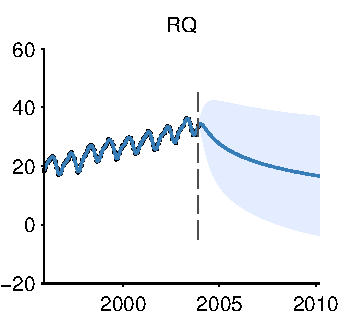
\includegraphics[width=0.11\textwidth]{../figures/11-Feb-v4-03-mauna2003-s_max_level_0/03-mauna2003-s_all_small.pdf} &
        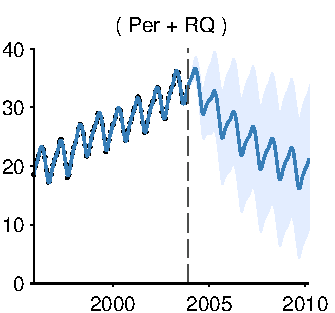
\includegraphics[width=0.11\textwidth]{../figures/11-Feb-v4-03-mauna2003-s_max_level_1/03-mauna2003-s_all_small.pdf} &
        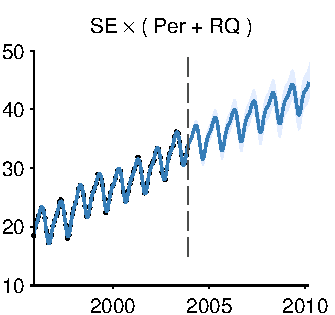
\includegraphics[width=0.11\textwidth]{../figures/11-Feb-v4-03-mauna2003-s_max_level_2/03-mauna2003-s_all_small.pdf} &
        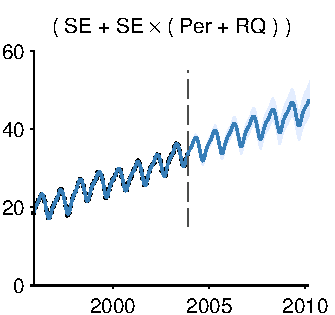
\includegraphics[width=0.11\textwidth]{../figures/11-Feb-v4-03-mauna2003-s_max_level_3/03-mauna2003-s_all_small.pdf}
\end{tabular}  
\end{center}

\vspace{1\baselineskip}

%\mysection{Example: Mauna Loa CO$_2$ concentration}
\mysection{Compound Kernels are Interpretable}

\vspace{0\baselineskip}

\begin{itemize}
  \item Compound kernels decompose functions into additive components% (additive components of the kernel correspond to independent additive functions)
\end{itemize}


%\begin{tikzpicture}[transform canvas={scale=0.75}] 
  \begin{scope}[yshift=0\textwidth]
    \begin{scope}[xshift=0cm]
      \node [mybox] (all) at (0, 0) {
        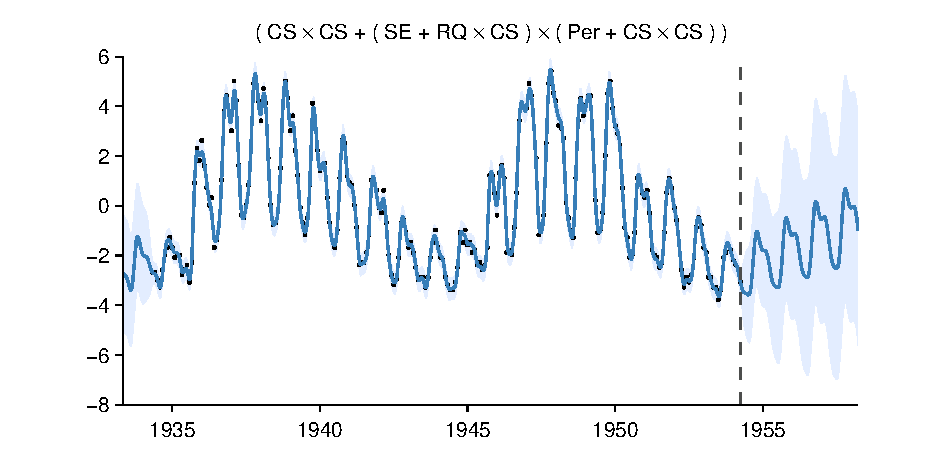
\includegraphics[width=0.23\textwidth]{../figures/radio/monthly-critical-radio-frequenci_all.pdf}
      };
    \end{scope}
  \end{scope}
  \begin{scope}[yshift=0\textwidth]
    \begin{scope}[xshift=0cm]
    \end{scope}
  \end{scope}
  \begin{scope}[yshift=-0.07\textwidth]
    \begin{scope}[xshift=0cm]
        \node [mybox, below of=all] (equals) at (0, 0) {\Huge{$=$}};
    \end{scope}
  \end{scope}
  \begin{scope}[yshift=-0.13\textwidth]
    \begin{scope}[xshift=-0.08\textwidth]
      \node [mybox] (all) at (0, 0) {
        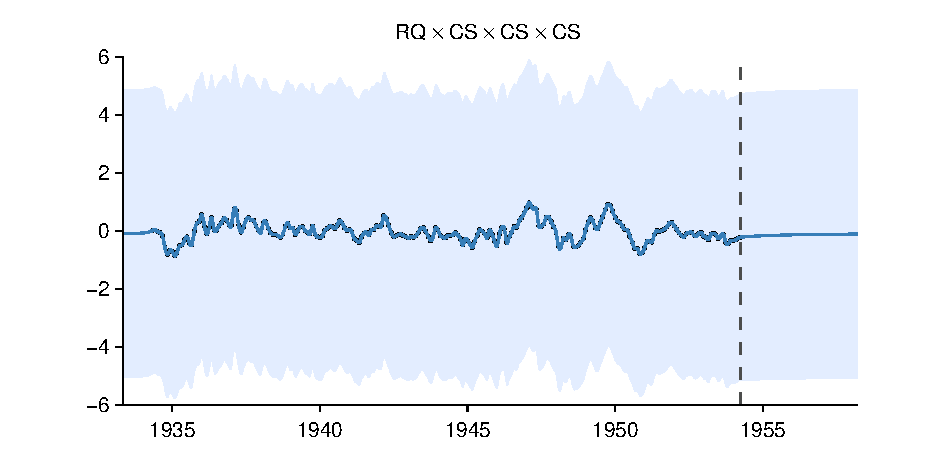
\includegraphics[width=0.13\textwidth]{../figures/radio/monthly-critical-radio-frequenci_5.pdf}
      };
    \end{scope}
    \begin{scope}[xshift=+0.08\textwidth]
      \node [mybox] (all) at (0, 0) {
        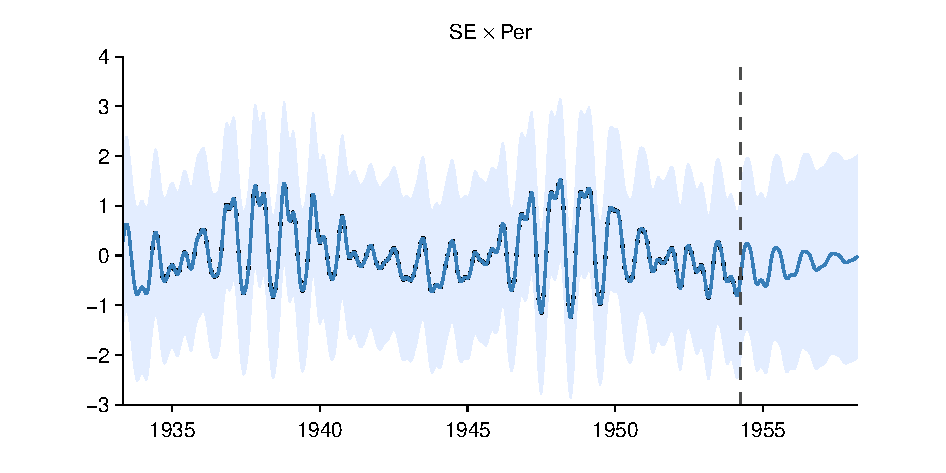
\includegraphics[width=0.13\textwidth]{../figures/radio/monthly-critical-radio-frequenci_2.pdf}
      };
    \end{scope}
  \end{scope}
  \begin{scope}[yshift=-0.17\textwidth]
    \begin{scope}[xshift=0cm]
        \node [mybox, below of=all] (equals) at (0, 0) {\Huge{+}};
    \end{scope}
  \end{scope}
  \begin{scope}[yshift=-0.22\textwidth]
    \begin{scope}[xshift=-0.08\textwidth]
      \node [mybox] (all) at (0, 0) {
        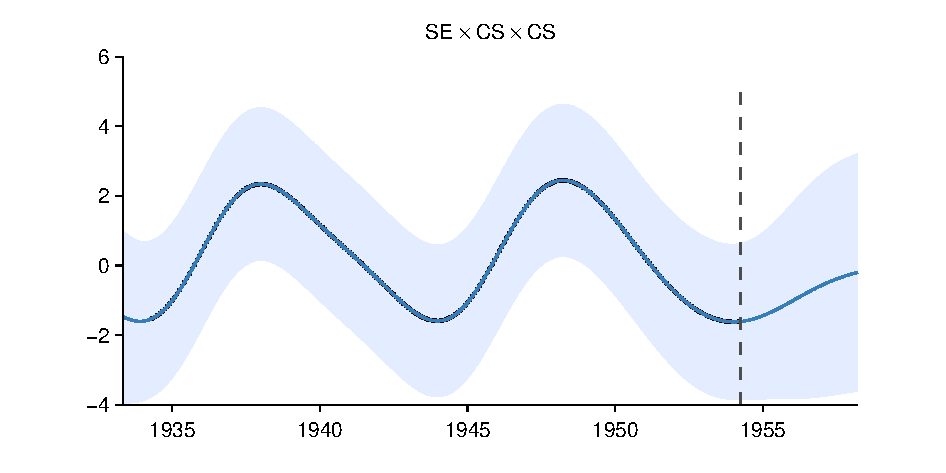
\includegraphics[width=0.13\textwidth]{../figures/radio/monthly-critical-radio-frequenci_3.pdf}
      };
    \end{scope}
    \begin{scope}[xshift=+0.08\textwidth]
      \node [mybox] (all) at (0, 0) {
        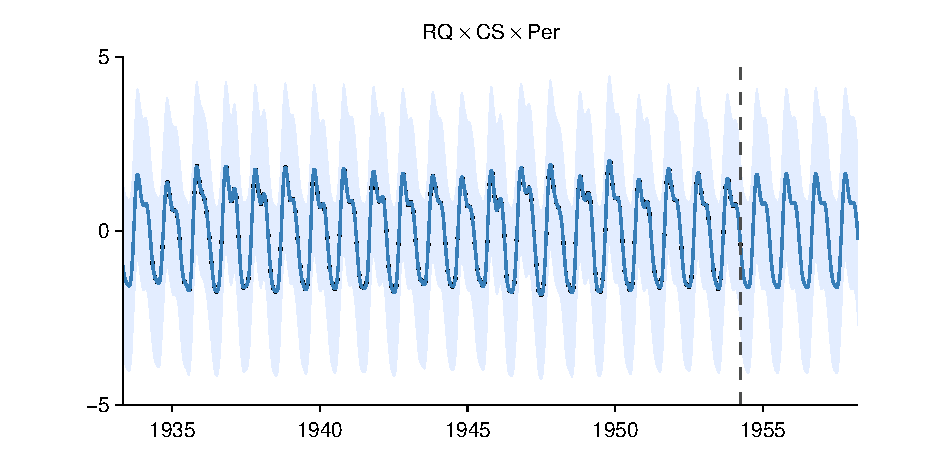
\includegraphics[width=0.13\textwidth]{../figures/radio/monthly-critical-radio-frequenci_4.pdf}
      };
    \end{scope}
  \end{scope}
\end{tikzpicture}

%\vspace{14\baselineskip}

%\vspace{14\baselineskip}
%\begin{tikzpicture}[transform canvas={scale=0.75}] 
  \begin{scope}[yshift=0.1\textwidth]
    \begin{scope}[xshift=-0.2\textwidth]
      \node [mybox] (all) at (0, 0) {
        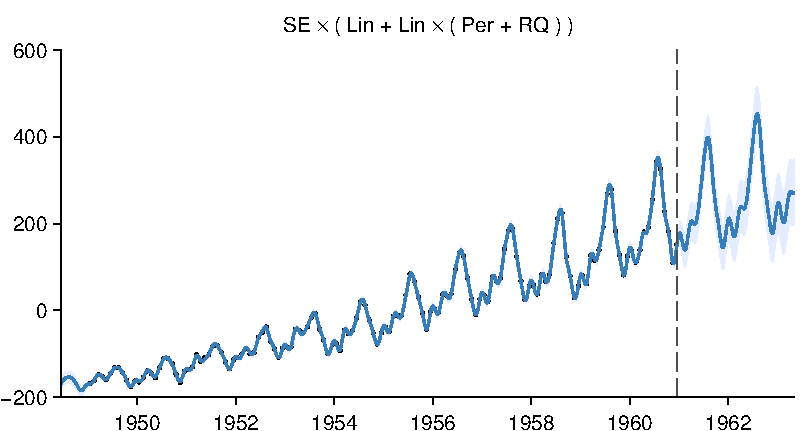
\includegraphics[width=0.25\textwidth]{../figures/01-airline-months_all.pdf}
      };
    \end{scope}
  \end{scope}
  \begin{scope}[yshift=0\textwidth]
    \begin{scope}[xshift=0cm]
    \end{scope}
  \end{scope}
  \begin{scope}[yshift=0.15\textwidth]
    \begin{scope}[xshift=0cm]
        \node [mybox, below of=all] (equals) at (0, 0) {\Huge{$=$}};
    \end{scope}
  \end{scope}
  \begin{scope}[yshift=-0\textwidth]
    \begin{scope}[xshift=0.05\textwidth]
      \node [mybox] (all) at (0, 0) {
        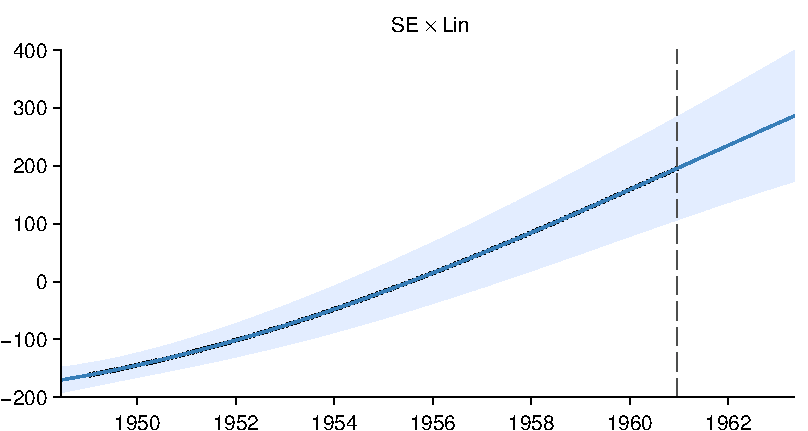
\includegraphics[width=0.2\textwidth]{../figures/01-airline-months_1.pdf}
      };
    \end{scope}
    \begin{scope}[xshift=+0.25\textwidth]
      \node [mybox] (all) at (0, 0) {
        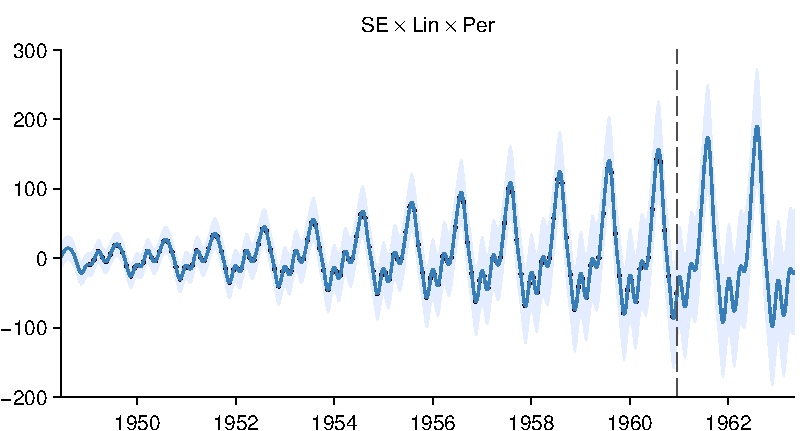
\includegraphics[width=0.2\textwidth]{../figures/01-airline-months_2.pdf}
      };
    \end{scope}
  \end{scope}
  \begin{scope}[yshift=0.1\textwidth]
    \begin{scope}[xshift=0cm]
        \node [mybox, below of=all] (equals) at (0, 0) {\Huge{+}};
    \end{scope}
  \end{scope}
  \begin{scope}[yshift=0.2\textwidth]
    \begin{scope}[xshift=0.05\textwidth]
      \node [mybox] (all) at (0, 0) {
        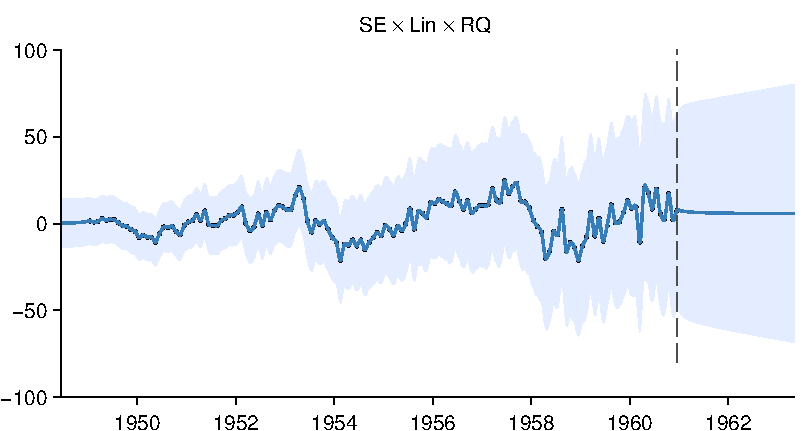
\includegraphics[width=0.2\textwidth]{../figures/01-airline-months_3.pdf}
      };
    \end{scope}
    \begin{scope}[xshift=+0.25\textwidth]
      \node [mybox] (all) at (0, 0) {
        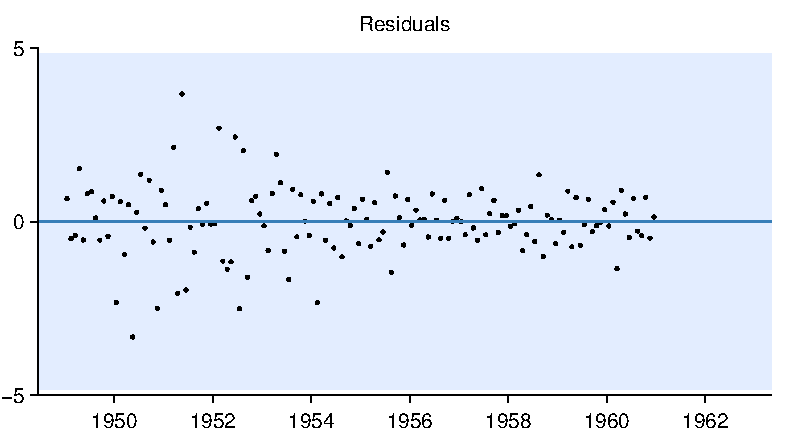
\includegraphics[width=0.2\textwidth]{../figures/01-airline-months_resid.pdf}
      };
    \end{scope}
  \end{scope}
\end{tikzpicture}


%\hline

\paragraph{\large Example: Airline passengers }

\vspace{1\baselineskip}

\newcommand{\postdw}{0.13\textwidth}  % Poster decomp width

\begin{tabular}{cc}
\begin{tabular}{c}
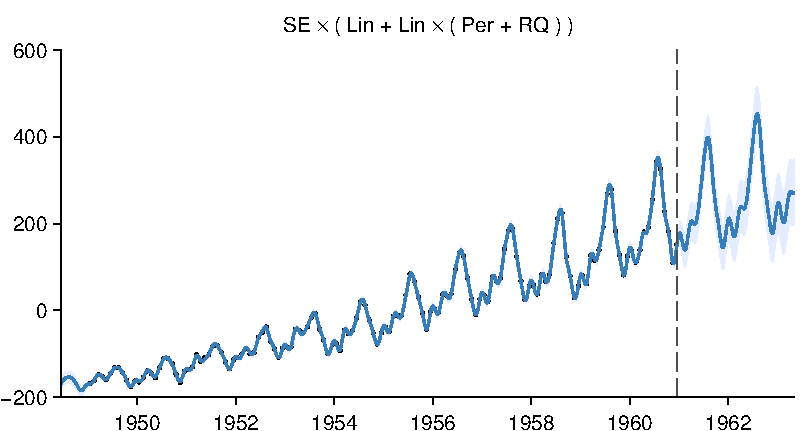
\includegraphics[width=0.2\textwidth]{../figures/01-airline-months_all.pdf}
\end{tabular} &
\begin{tabular}{cc}
%Monthly airline traffic decomposes into a sum of:}\\
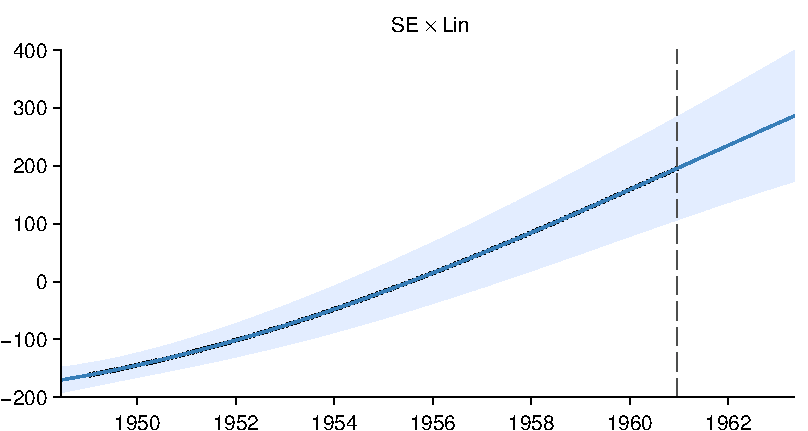
\includegraphics[width=\postdw]{../figures/01-airline-months_1.pdf} &
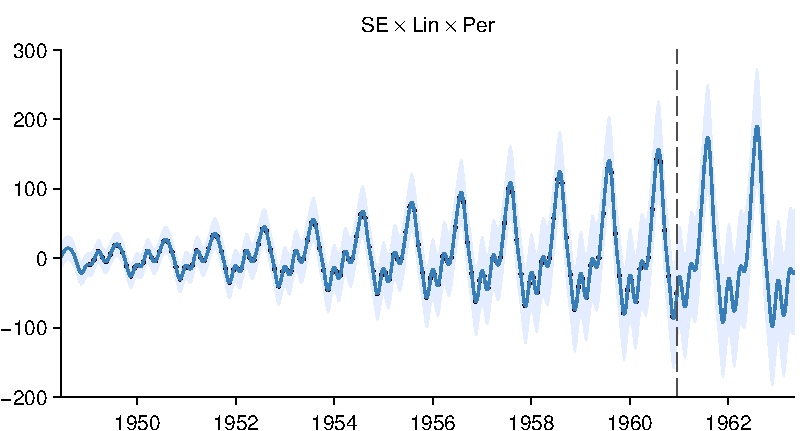
\includegraphics[width=\postdw]{../figures/01-airline-months_2.pdf} \\
Long-term trend & Growing amplitude \\
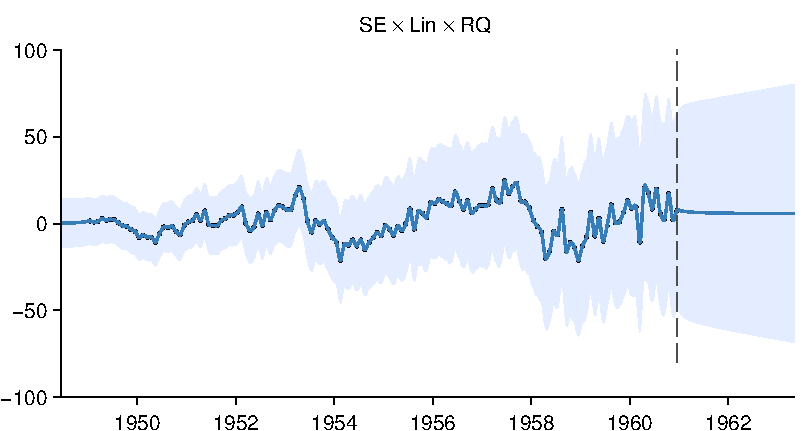
\includegraphics[width=\postdw]{../figures/01-airline-months_3.pdf} &
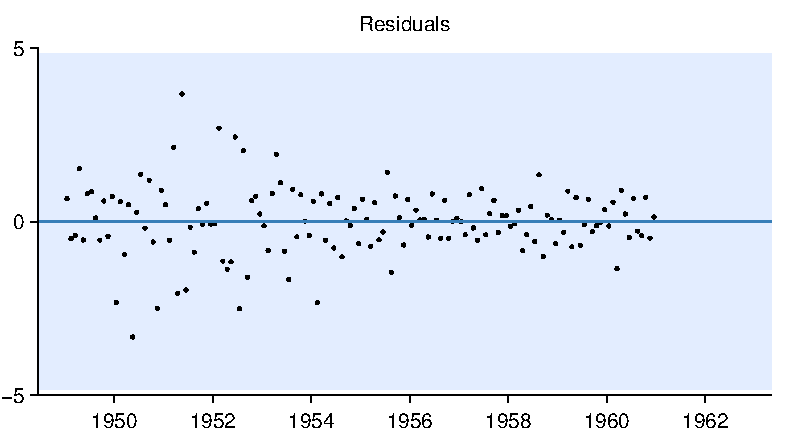
\includegraphics[width=\postdw]{../figures/01-airline-months_resid.pdf} \\
Short-term deviatinos & noise \\
%Smooth long-term trend + \quad %
%Linearly growing periodic + \quad &
%Short-term deviations
\end{tabular}
\end{tabular}
% QR code
%\def \badgeheight {0.08\textwidth}
%
\includegraphics[height=\badgeheight]{../badges/QR.png}

%\hline

\paragraph{\large Example:  Radio usage }

\vspace{1\baselineskip}

\begin{tabular}{cc}
\begin{tabular}{c}
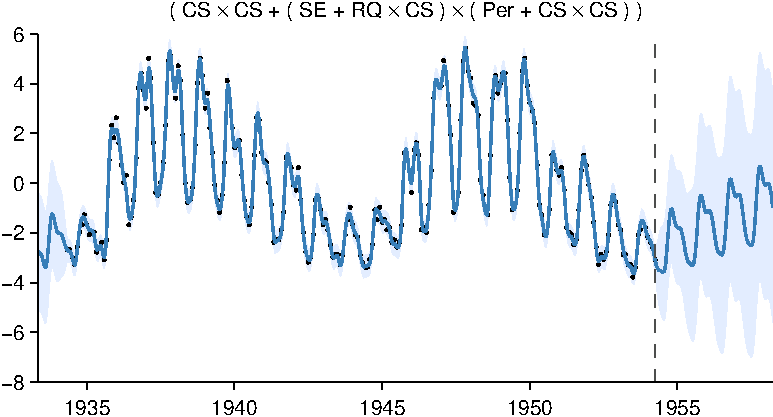
\includegraphics[width=0.2\textwidth]{../figures/radio/all.pdf}
\end{tabular} &
\begin{tabular}{cc}
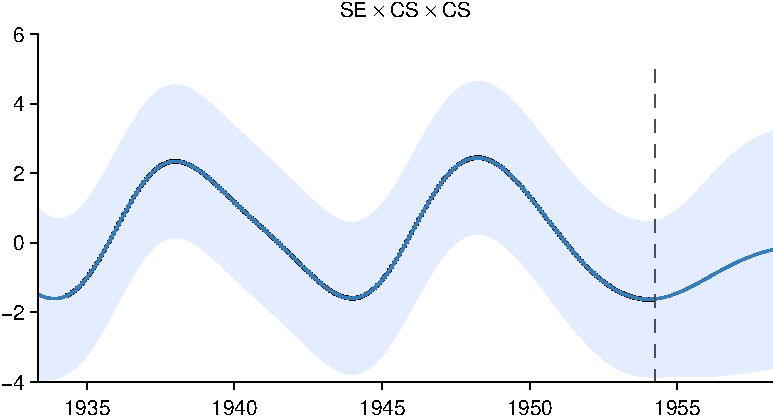
\includegraphics[width=\postdw]{../figures/radio/3.pdf} &
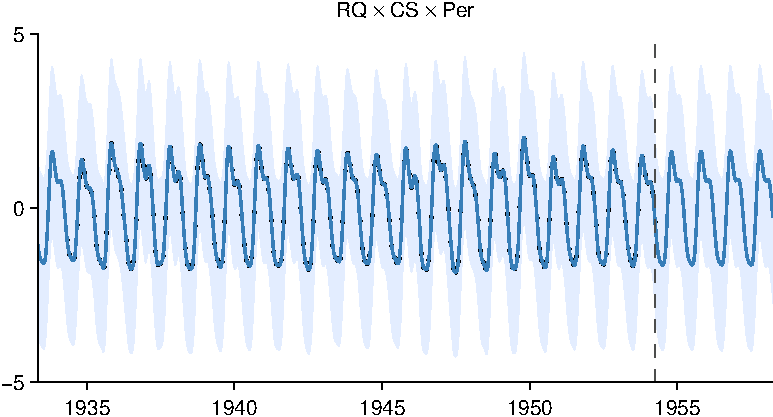
\includegraphics[width=\postdw]{../figures/radio/4.pdf} \\
Long-term smooth + \quad &
Yearly priodic \\
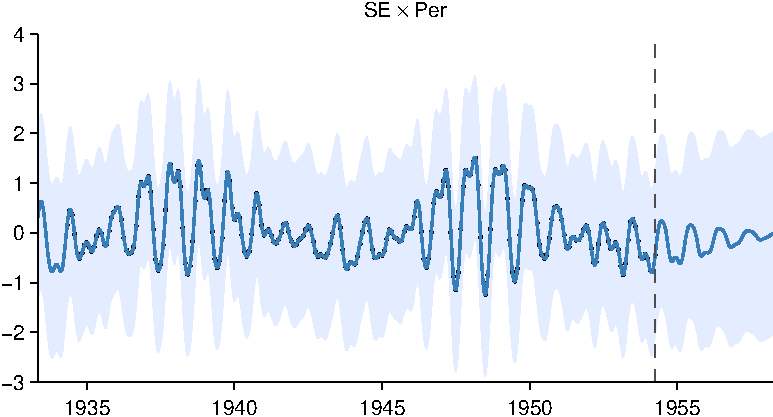
\includegraphics[width=\postdw]{../figures/radio/2.pdf} &
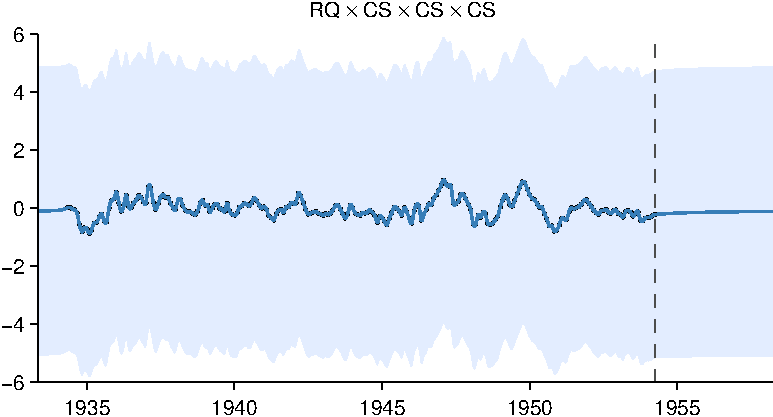
\includegraphics[width=\postdw]{../figures/radio/5.pdf} \\
Long-term amlpitude + \quad &
Short-term noise \quad
\end{tabular}
\end{tabular}

    % QR code
    %\node [mybox] (QR code) at (-0.95, 0) {

 \vfill
 
 %Code available at \href{http://www.github.com/jamesrobertlloyd/gp-structure-search}
 
    \hfill    
\includegraphics[height=6cm]{../badges/QR.png}

\end{multicols}

\end{poster}

\end{document}

